% =====================================================================
%  SVD-TA / Compressed Traffic Assignment -- manuscript v3
%  Numerical-rerun pass: 2026-07-24   (repro code: CompressedTAP @ 2adc6d4, branch version_3)
%  Re-evaluated this pass : Table 2 (Sioux consistency); Table 4 Panel A -- Chicago Sketch
%                           (all tau) and Philadelphia (tau = 0, 0.67).
%  NOT re-evaluated (--)  : Panel A Chicago Regional; Table 5 (rank); Table 4 Panel B.
%  C++/Python metrics verified CONSISTENT on the Sketch instance
%  (Gap_F within 0.03pp, R^2 within 1.2e-3).
% =====================================================================
\documentclass[11pt]{article}
\usepackage{amsfonts,amsmath,amsthm,amssymb}
\usepackage{graphicx}
\usepackage{booktabs}
\usepackage{float}
\usepackage{longtable}
\usepackage{geometry}
\usepackage[table]{xcolor}
\usepackage{url}
\usepackage[normalem]{ulem}

% Conservative revision markup: unchanged submitted text remains black;
% proposed replacements/additions are red.
\newcommand{\revnote}[1]{\par\noindent{\color{red}\textbf{Revision note:} #1}\par}


\newtheorem{exmp}{Example}[section]
\newtheorem{theorem}{Theorem}[section]
\newtheorem{lemma}[theorem]{Lemma}
\newtheorem{proposition}[theorem]{Proposition}
\newtheorem{remark}{Remark}[section]
\newtheorem{corollary}[theorem]{Corollary}
\newtheorem{definition}[theorem]{Definition}
\newtheorem{conjecture}[theorem]{Conjecture}
\newtheorem{axiom}[theorem]{Axiom}
\newtheorem{assumption}{Assumption}[section]

\title{Compressed Traffic Assignment with the \\Augmented Lagrangian Method\footnote{
This work was carried out at the Fulton School of Engineering, Arizona State University, Tempe, AZ. X. Zhou and Y. Li are with School of Sustainable Engineering and the Built Environment, ASU. P. Li is with Norfolk Southern Corporation. D. Bertsekas is with School of Computing and Augmented Intelligence, ASU.}}
\author{Xuesong Zhou, Peiheng Li, Yuchao Li, and Dimitri Bertsekas}
\date{April 2026}

% ---- draft version stamp (bump DOCVER on every circulated build) ----
\newcommand{\docver}{v3.5}
\newcommand{\docdate}{2026-07-25}
\newcommand{\doccommit}{0077beb}
\newcommand{\docstamp}{Draft \docver\ \textbullet\ built \docdate\ \textbullet\ code
  \texttt{CompressedTAP@\doccommit} (\texttt{version\_3}) \textbullet\ numerical section
  rewritten; flow-weighted basis; paired-comparison figures; body in black, red = notes to co-authors}

% Author-facing notes (red). \shownotesfalse suppresses them for a submission build;
% the calls can then stay in the source.
\newif\ifshownotes \shownotestrue
\newcommand{\conote}[1]{\ifshownotes{\color{red}\small\textsf{[Note to co-authors: #1]}}\fi}
\newcommand{\conoteY}[1]{\ifshownotes{\color{red}\small\textsf{[Note to Yuchao: #1]}}\fi}

\begin{document}
\maketitle
\begin{center}\small\textsf{\docstamp}\end{center}

\begin{abstract}
{\color{red}
We consider large-scale traffic assignment problems and develop an integrated major--minor path-compression and solution framework. Paths are partitioned according to nominal flows and a prescribed threshold: major paths are retained explicitly, while deviations of the minor-path flows from their nominal values are represented in a truncated singular-vector subspace of the minor path--link incidence matrix. A simple safeguard preserves feasibility, and the resulting lower-dimensional convex formulation is solved by an augmented Lagrangian method with separate penalty parameters for the equality and reconstructed nonnegativity constraints. The contribution is this integrated compression-and-solution framework; neither singular value decomposition nor the augmented Lagrangian principle is proposed in isolation.

We report computational studies using the Chicago Sketch, Chicago Regional, and Philadelphia networks. The revised experiments use a consistently converged uncompressed formulation as the primary reference and report preprocessing separately from the online augmented Lagrangian solution time. The results characterize a dimension--accuracy--computation trade-off: moderate compression can reduce the number of optimization variables and the cost per inner iteration while maintaining high link-flow fidelity, but total-time gains are problem-dependent because the reconstructed minor-path nonnegativity constraints retain path-scale operations. The framework is therefore intended for related or repeated assignment calculations in which a path pool and nominal flow information are already available and the one-time compression effort can be reused.
}
\end{abstract}

%% ======================================================================
%% SECTION 1: INTRODUCTION
%% ======================================================================
\section{Introduction}\label{sec:intro}
The traffic assignment problem is a classical problem in transportation science and network optimization. In its standard user-equilibrium formulation, it can be posed as a convex optimization problem that distributes travel demand across network paths subject to flow conservation and nonnegativity constraints. This formulation goes back to the seminal work of \cite{beckmann1956studies}, and it has motivated a large literature on both modeling and computation. In particular, the Frank-Wolfe method \cite{frank1956algorithm} became a standard approach because it avoids exhaustive path enumeration by solving shortest-path subproblems iteratively. Subsequent developments, including gradient projection, quasi-Newton, and conjugate-direction methods, have improved computational performance substantially; see, for example, \cite{jayakrishnan1994fast}, \cite{bertsekas1980class, bertsekas2011centralized}, \cite{mitradjieva2013stiff}, and the textbook treatments in \cite{sheffi1985urban, ahuja1993network, patriksson1994traffic, bertsekas1998network, boyles2020transportation}.

Despite this progress, path-based formulations remain difficult to solve at large scale because the number of feasible paths can be enormous. As network size grows, the associated path-link incidence matrix becomes very large, and the resulting optimization problem becomes increasingly expensive in both storage and computation. Existing methods alleviate this difficulty in different ways, for example, by generating paths selectively, refining active path sets, or exploiting origin-based structure. However, they do not directly reduce the dimension of the underlying path space. This dimensionality challenge is the starting point of the present work.

Our approach is motivated by a simple structural observation: in many realistic traffic assignment problems, \emph{only a relatively small subset of paths carries substantial flow, while many other paths make smaller contributions to the aggregate link flows}. This suggests that the full path space may contain substantial redundancy from the standpoint of optimization. We exploit this structure by partitioning the paths into two groups. The first group consists of \emph{major paths}, which are retained explicitly as decision variables. The second group consists of \emph{minor paths}, whose contribution is represented approximately in a low-dimensional subspace obtained from a truncated singular value decomposition (SVD) of the corresponding minor-path submatrix of the path-link incidence matrix.

The proposed framework is aimed primarily at applications where closely related large-scale traffic assignment problems must be solved repeatedly. In such cases, nominal path-flow information from a previous solution, a nearby scenario, or a coarse preliminary calculation can be used to identify the major paths that should be retained explicitly. This information need not be exact; its role is only to guide the major-minor partition. Thus, our framework is not intended to replace a one-time full solve from scratch, but to exploit reusable nominal information in order to accelerate the solution of related instances.\par
{\color{red}The path pool is treated as an input to the compressed formulation. Accordingly, the paper does not propose a replacement for path generation or claim that compression is preferable for every traffic assignment calculation; it studies whether an already available path-based formulation can be reduced before repeated optimization.}

Our construction yields a compressed path-based formulation with substantially fewer variables than the original problem. At the same time, the compressed problem preserves the basic convex structure of the original formulation. We also incorporate a simple safeguard that ensures feasibility of the compressed formulation whenever the original problem is feasible. Thus, the proposed method is more than a heuristic compression scheme: it yields a well-defined convex optimization problem that preserves the essential structure of the original traffic assignment model.

{\color{red}To solve the compressed problem, we use an augmented Lagrangian (AL) method with separate penalty parameters for the equality and reconstructed nonnegativity constraints. The paper is organized around one contribution: a nominal-flow-informed major--minor compression framework whose affine SVD representation and AL solution procedure are two inseparable components of the same construction. The AL principle is standard in isolation; its role here is to provide a reliable solution mechanism for the specific compressed formulation.}

The remainder of the paper is organized as follows. In Section~\ref{sec:background}, we review related work on traffic assignment algorithms, spectral methods in transportation, and reduced-order convex programming. In Section~\ref{sec:compression_framework}, we develop the compressed formulation and establish its feasibility and approximation properties. In Section~\ref{sec:alm}, we describe the AL method and its algorithmic properties. In Section~\ref{sec:experiments}, we report our computational studies on three networks. Section~\ref{sec:conclusion} concludes and discusses broader implications.

%% ======================================================================
%% SECTION 2: BACKGROUND AND RELATED WORK
%% ======================================================================
\section{Background and Related Work}\label{sec:background}

In this section, we review three strands of literature most relevant to our work. We first discuss path-based traffic assignment algorithms and their computational limitations at large scale. We then examine spectral and rank-based ideas in transportation, emphasizing the distinction between algebraic rank and the optimization-oriented use of truncated SVD in our framework. Finally, we discuss the connection between our approach and the broader literature on reduced-order convex optimization.

\subsection{Traffic Assignment Problem and Solution Algorithms}

Path-based formulations of the traffic assignment problem have been studied extensively, but their central computational difficulty has remained the same: the number of feasible paths can be extremely large, and the associated path--link incidence matrix grows rapidly with network size. This creates substantial challenges in both storage and computation for realistic transportation networks.

A classical way to address this difficulty is to avoid full path enumeration. The Frank-Wolfe algorithm and its variants generate shortest paths iteratively and have long served as standard methods for solving traffic assignment problems. Other path-based approaches, including gradient projection, conjugate-gradient-type methods, and Newton-type methods, improve computational performance by refining active path sets and exploiting the smooth structure of the objective. These methods have substantially advanced the computational treatment of traffic assignment, but they still operate in the original high-dimensional path space.

Another line of work improves tractability by exploiting network structure. Origin-based and bush-based methods, have originated in both data and transportation network research, and organize computations around origins or acyclic subnetworks \cite{gallager1977minimum,bertsekas1984second,bar2002origin,nie2010class}. Other approaches use greedy path management, decomposition, or operator-splitting techniques such as ADMM to improve scalability \cite{xie2018greedy, yao2019admm, liu2023alternating, liu2024novel, liu2025admm}. Mesoscopic and cross-resolution modeling frameworks \cite{zhou2014dtalite, zhou2022meso}, together with open-source tools such as \texttt{Path4GMNS} \cite{Path4GMNS} and \texttt{AequilibraE} \cite{camargo2015aequilibrae}, have further improved the practical study of large-scale traffic assignment problems.

However, these approaches primarily seek to manage or decompose the original path space rather than reduce its dimension directly. By contrast, our focus is on constructing a compressed path-based formulation in which the dimension of the decision space itself is reduced. In this sense, our approach is complementary to existing traffic assignment algorithms: rather than proposing another method for the full path representation, we reformulate that representation so that the resulting optimization problem is smaller.

\subsection{Spectral Methods and Rank Structure in Transportation}

Spectral and low-rank ideas have appeared in transportation in several different contexts. Early work used SVD and principal component analysis to support dynamic traffic assignment and online calibration \cite{peeta1999generalized, prakash2017reducing}. Other studies examined the rank of the path--link incidence matrix from the standpoint of observability, sensor placement, and network reconstruction \cite{hu2009identification, zhou2010information}. In these works, rank is interpreted in the algebraic sense, namely, as the number of linearly independent rows or columns needed to represent the matrix exactly.

This algebraic interpretation also relates to methods such as column generation and Dantzig-Wolfe decomposition, where linearly independent columns are generated so that the original constraint system is satisfied exactly in the limit, as the number of generated columns increases \cite{lubbecke2005selected, barnhart1998branch}. Our use of spectral structure is different. We do not use SVD to identify an exact basis for the path space, nor do we rely on rapid singular-value decay to justify compression from a matrix-approximation viewpoint alone. Instead, we use truncated SVD as a device for constructing a lower-dimensional representation of the contribution of minor paths to aggregate link flows.

This distinction is important for the present paper. In our experiments, the singular values of the minor-path incidence matrix decay gradually rather than rapidly. Thus, the matrix is not strongly low-rank in the usual spectral reconstruction sense. Nevertheless, moderate-rank compression still performs well in the optimization problem: it preserves high link-flow fidelity and yields useful reductions in computational cost. This indicates that the effectiveness of the compression is governed less by accurate reconstruction of the minor-path matrix itself than by the relative insensitivity of the optimization problem to higher-order components of the minor-path representation.

Most recently, \cite{zhang2025lowrank} constructed reduced hypothetical path sets with real-valued (non-binary) path--link incidence matrices by fitting a surrogate Logit-based stochastic user equilibrium model. Their approach provides evidence of low-dimensional structure in path-based traffic models, but it differs from ours in both objective and construction: they replace the original assignment model with a surrogate one, whereas we compress the original binary incidence matrix directly and solve a reduced formulation of the original Beckmann problem.

\subsection{Reduced-Order Convex Programming}

Low-rank reduction is also a common idea in large-scale optimization. In many problems, a high-dimensional model admits an effective lower-dimensional representation that preserves the components most relevant to the optimization objective while reducing computational cost. Such ideas appear in areas such as portfolio optimization \cite{markowitz1952portfolio, ross1976arbitrage, chopra1993effect}, machine learning \cite{vapnik1995nature, scholkopf1998nonlinear, rahimi2008random}, matrix approximation \cite{eckart1936approximation, golub1965svd, sirovich1987low, sarwar2000application, koren2009matrix, candes2009exact}, and aggregation in approximate dynamic programming \cite{bertsekas2012dynamic,bertsekas2019reinforcement}.

Our work brings this reduced-order viewpoint to path-based traffic assignment. The key idea is to introduce low-rank representation not in observed traffic data, but in the path-based incidence matrix that defines the optimization problem itself. By projecting the minor-path component onto a low-dimensional spectral subspace, we obtain a reduced-order convex program that remains closely connected to the original traffic assignment model while involving substantially fewer decision variables.

This perspective places our work at the intersection of path-based traffic assignment and reduced-order convex optimization. The resulting formulation preserves convexity and, under a natural structural condition, feasibility as well. It can then be solved effectively by an AL method designed for the compressed structure.



\section{Problem Formulation and Path-Based Compression}\label{sec:compression_framework}

In this section, we describe our path-based compression method. We start by introducing the classical traffic assignment problem. We then introduce our compression framework, and provide a condition under which the compressed problem remains feasible.



%%%%%%%%%%%%%%%%%%%%%%%%%%%%%%%%%%%%%%%



\subsection{Traffic Assignment Problem}
We consider a transportation network with $m$ directed links, $n$ paths, and $\ell$ origin-destination (OD) pairs. Let $A$ be the $\ell$ by $n$ OD-path incidence matrix (rows correspond to OD pairs, and  columns correspond to paths, with entries being either 1 or 0, depending on whether the column path corresponds to  the row OD pair, or not). Let $B$ be the $n$ by $m$ path-link incidence matrix (rows correspond to paths, and  columns correspond to links, with entries being either 1 or 0, depending on whether  the row path contains the column link, or not). There is a given nonnegative OD pair demand vector $d\in \Re^\ell$. There is also a given nonnegative offset link flow vector $v_0$. In particular, the vector $v_0$ can represent the known contributions to the link flows by the OD pairs that have a unique path from origin to destination. 



The traffic assignment problem is defined as
\begin{equation}
    \label{eq:original_ta}
    \begin{aligned}
        \min_{x,v}\quad & f(v)\\
    \text{s.t.}\quad &v=B'x+v_0,\ \ Ax=d, \ \ x\geq 0,
    \end{aligned}
\end{equation}
where $f$ is a given convex function of the link flow vector $v$ [specifically, the Bureau of Public Roads (BPR) congestion cost in our numerical experiments], a prime denotes transposition, and the inequality $\geq$ is meant to be component-wise. 

Implicit in our formulation is that each OD pair has at least one path and that each path belongs to exactly one OD pair, so the problem is feasible, the matrix $A$ has rank $\ell$, and each column of $A$ is a column of the $\ell\times \ell$ identity matrix.    
Since the cost function $f$ is convex and the constraints are linear, problem \eqref{eq:original_ta} is a convex programming problem.

Despite being convex and feasible, problem \eqref{eq:original_ta} can be challenging to solve. This is because the values of $n$ and $\ell$ are often quite large for practical problems. We will next introduce a compressed problem, which involves fewer variables, thus facilitating its computational solution.





\subsection{Path Compression and Compressed Problem}
\label{sec:compression}

In many practical contexts, nominal path-flow information is often available from historical data, prior computations, or coarse preliminary solutions, and can be used to identify the paths that are likely to be dominant. These are the \emph{major paths} that have significant impact on the link flows $v$. In contrast, the remaining paths can be regarded as \emph{minor paths}, whose contributions to the link flows are secondary. Our approach is to approximate the contributions of the minor paths to the link flows via SVD, as we discuss next.

In particular, let $\tau$ be a threshold on the nominal flow. For OD pairs that have multiple corresponding paths,  we select major paths according to the following two rules:
\begin{itemize}
    \item[1)] For each OD pair, the path that has the largest nominal flow is a major path; 
    \item[2)] The remaining paths are split into major paths (those with nominal flow bigger than $\tau$) and minor paths (those with nominal flow no more than $\tau$).  
\end{itemize}

The first rule ensures that the OD conservation constraints remain solvable under compression. We will discuss this in Section~\ref{sec:convex_feasible}. The second rule allows us to use our knowledge of a nominal flow to simplify the problem. 

Without loss of generality, let us assume that the first $s$ elements of the vector $x$ correspond to the major paths. As a result, we can partition the vector $x$ as
$$x=\begin{pmatrix}
    y\\
    w
\end{pmatrix},$$
where $y\in \Re^s$ and $w\in \Re^{n-s}$ represent the flows of the major and minor paths, respectively. Accordingly, we can partition the matrix $B$ as
$$B=\begin{pmatrix}
    B_1\\
    B_2
\end{pmatrix},$$
where the dimensions of $B_1$ and $B_2$ are $s$ by $m$ and $(n-s)$ by $m$, respectively. Suppose that $B_2$ is approximated via SVD as
$$B_2\approx U_r\Sigma_r V_r',$$
where $U_r$ is an $(n-s)$ by $r$ matrix, and the dimensions of $\Sigma_r$ and $V_r$ are determined accordingly. The value $r$ is a design parameter, which represents the extent to which the matrix $B_2$ is approximated.


{\color{red}
By the Eckart--Young theorem, this truncated SVD is the best rank-$r$ approximation of $B_2$ in the spectral norm; see \cite[Theorem~2.4.8]{golub2013matrix}. Let the nominal minor-path flow be $w_0$. Then the link-flow approximation error associated with a deviation from the nominal flow satisfies
$$\big\|(B_2-U_r\Sigma_rV_r')'(w-w_0)\big\|\leq \sigma_{r+1}\|w-w_0\|,$$
where $\|\cdot\|$ denotes the Euclidean norm and $\sigma_{r+1}$ is the largest discarded singular value. We therefore approximate the minor-path flow by the affine representation
$$x=\begin{pmatrix}
    y\\
    w_0+U_rz
\end{pmatrix},$$
where $z\in\Re^r$. Thus, the nominal link-flow contribution $B_2'w_0$ is retained exactly, while the deviation $w-w_0$ is represented in the truncated singular-vector subspace. The matrix being decomposed remains $B_2$; only the minor-path flow representation is centered. The corresponding link flow is
\begin{align*}
    v=&B'x+v_0=(B_1'\;\;B_2')\begin{pmatrix}
    y\\
    w_0+U_rz
\end{pmatrix}+v_0\\
=&B_1'y+Dz+B_2'w_0+v_0,
\end{align*}
where $D=B_2'U_r$ is an $m$ by $r$ matrix.

Similarly, partition $A=(A_1\;A_2)$, where $A_1$ is an $\ell$ by $s$ matrix and $A_2$ is an $\ell$ by $(n-s)$ matrix. Then
$$Ax=A_1y+Mz+A_2w_0,$$
where $M=A_2U_r$, and nonnegativity becomes
$$y\geq0,\qquad w_0+U_rz\geq0.$$
Writing $\bar d=d-A_2w_0$, the compressed problem is
\begin{equation}
    \label{eq:compressed_ta}
    \begin{aligned}
        \min_{y,z}\quad & \hat f(y,z)\\
    \text{s.t.}\quad & y\geq0,\quad A_1y+Mz=\bar d,\quad w_0+U_rz\geq0,
    \end{aligned}
\end{equation}
where $\hat f(y,z)=f(B_1'y+Dz+B_2'w_0+v_0)$. Setting $w_0=0$ recovers the uncentered formulation in the submitted version. We summarize the main notation in Table~\ref{tab:notation} given in Appendix~\ref{app:notation}.
}




\subsection{Convexity and Feasibility of the Compressed Problem}\label{sec:convex_feasible}

As discussed earlier, the original problem is convex and  feasible. Clearly, we would like the compressed problem to remain convex and feasible. The convexity of the compressed problem follows directly from $f$ being convex and the constraints in \eqref{eq:compressed_ta} being linear; see e.g., \cite[Prop. 1.1.4]{bertsekas2009convex}. 

{\color{red}To see the feasibility of the affine compressed problem, suppose first that the nominal flow satisfies the OD demand constraints, so that there is a nominal major-path flow $y_0\geq0$ with $A_1y_0+A_2w_0=d$. Then $\bar d=A_1y_0\geq0$, and $(y,z)=(y_0,0)$ is feasible. If the nominal flow comes from a different demand, the nominal minor flows of any violating OD pair are proportionally reduced so that their total does not exceed that OD demand. This yields $\bar d\geq0$. Because at least one major path is retained for every OD pair, $A_1y=\bar d$ can then be satisfied by assigning $\bar d_i$ to one retained major path of OD pair $i$ and setting its remaining major-path flows to zero. Thus, a feasible point with $z=0$ always exists after this safeguard.}

We note that the classical Beckmann formulation often involves a cost function that is strictly increasing with the link flows. As a result, the optimal link flows are unique, but the optimal path flows are generally not. This non-uniqueness property is inherent to the problem structure and is neither introduced nor resolved by the compression. Since solution quality is determined by the link flows rather than the path flows, the compressed formulation can achieve high fidelity without recovering individual minor-path flows.

Figure~\ref{fig:compression-pipeline} summarizes the six steps of our compression procedure, from the original problem with $n+m$ variables to the reduced formulation with $s + r$ variables.

\begin{figure}[htbp]
\centering
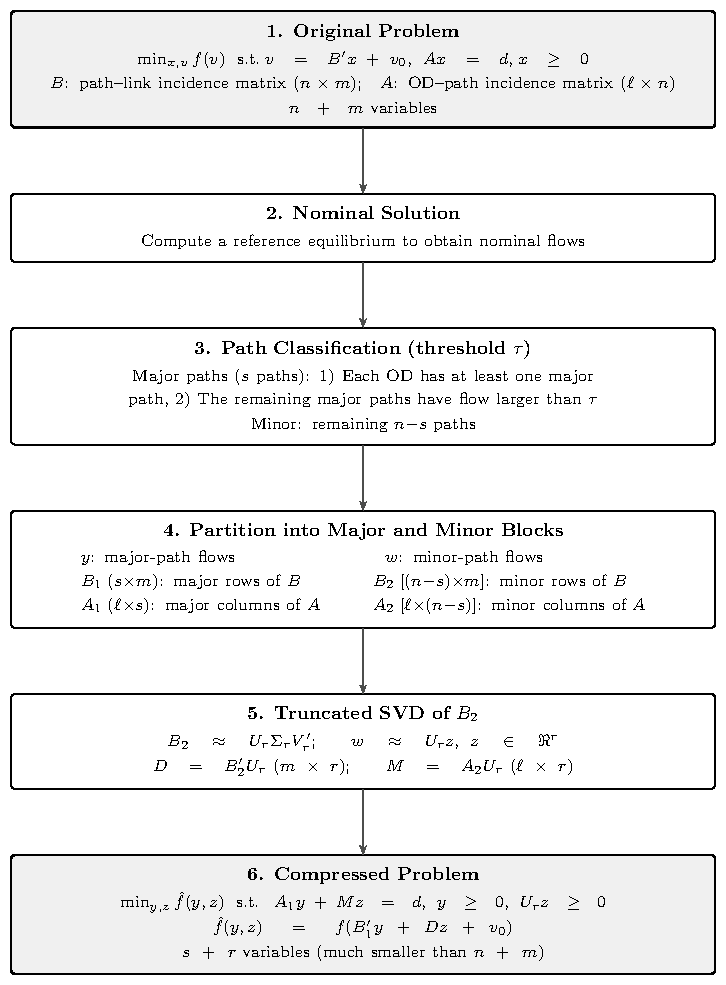
\includegraphics[width=0.8\textwidth]{fig/fig_compression_pipeline.pdf}
\caption{Architecture of the major--minor path compression framework.
A nominal solution partitions paths into major (retained) and minor
(compressed via truncated SVD of $B_2$), yielding a formulation with
$s + r$ variables, which can be a lot less than the $n+m$ variables of the original problem.}
\revnote{In the final clean figure, replace $w\approx U_rz$ by $w\approx w_0+U_rz$ and update the Step 6 equality, nonnegativity constraint, and objective consistently. No other architectural change to the figure is proposed.}
\label{fig:compression-pipeline}
\end{figure}

%% ======================================================================
%% SECTION 4: AUGMENTED LAGRANGIAN METHOD
%% ======================================================================
\section{Solution via the Augmented Lagrangian Method}
\label{sec:alm}
We solve problem \eqref{eq:compressed_ta} via the AL method with partial elimination of constraints; see, e.g., \cite[Section 2.4]{Ber82a}, \cite[Section~5.2]{bertsekas2016nonlinear}. There are two reasons for this choice. First, the AL method is known to be reliable and enables the use of efficient computational tools for optimization problems with simple inequality constraints, such as $x\ge0$ and $y\ge0$. Second, solutions from previous iterations in the AL method can be used to facilitate the computation of subsequent iterations. These features make the AL method well-suited for addressing the compressed problem \eqref{eq:compressed_ta}. In what follows, we describe the exact AL method that we use, including the AL function and multiplier update formulas for each iteration.

\subsection{Augmented Lagrangian Function}
We denote by $\lambda$ and $\mu$ the multipliers associated with the constraints \textcolor{red}{$A_1 y + M z - \bar d = 0$ and $w_0+U_r z \geq 0$}, respectively. As a result, we have $\lambda\in \Re^\ell$ and $\mu\in \Re^{n-s}$. For these two sets of constraints, we also associate different penalty parameters, which define a two-dimensional vector $c$, i.e., $c = (c_1, c_2)$, where $c_1$ and $c_2$ are associated with the constraints \textcolor{red}{$A_1 y + M z - \bar d = 0$ and $w_0+U_r z \geq 0$}, respectively. We will also use the subscript $i$ to denote the $i$th component of a vector. In particular, \textcolor{red}{$[w_0+U_r z]_i$ is the $i$th component of the vector $w_0+U_r z$}. 

Using the notation introduced above, the AL function is given as:
\begin{equation}
    \label{eq:aug_lag_form_2}
    \begin{aligned}
            {L}_c(y,z,&\lambda,\mu)\\
    =&\hat f(y,z)+\lambda'(A_1y+Mz-\textcolor{red}{\bar d})+\frac{c_1}{2}\Vert A_1y+Mz-\textcolor{red}{\bar d}\Vert^2+\\
    &\ \ \frac{1}{2c_2}\sum_{i=1}^{n-s}\Big\{\big(\max\{0,\mu_i-c_2[\textcolor{red}{w_0+U_rz}]_i\}\big)^2-\mu_i^2\Big\}.
    \end{aligned}
\end{equation}

The function $L_c(y, z, \lambda, \mu)$ is continuously differentiable with respect to $y$ and $z$. The gradients are given by:
\begin{align*}
    \nabla_{y}{L}_c(y,z,\lambda,\mu)=&\nabla_{y}\hat f(y,z)+A_1'\big(\lambda+ c_1(A_1y+Mz-\textcolor{red}{\bar d})\big),\\
    \nabla_{z}{L}_c(y,z,\lambda,\mu)=&\nabla_{z}\hat f(y,z)+M'\big(\lambda+c_1(A_1y+Mz-\textcolor{red}{\bar d})\big)-
    U_r'\big(\mu+c_2h^+(z,\mu,c_2)\big),
\end{align*}
where
\begin{equation}
\label{eq:h_p_def}
    h^+(z,\mu,c_2)=\begin{pmatrix}
        h_1^+(z,\mu,c_2)\\
        h_2^+(z,\mu,c_2)\\
        \vdots\\
        h_{n-s}^+(z,\mu,c_2)
    \end{pmatrix},\qquad h_i^+(z,\mu,c_2)=\max\bigg\{-[\textcolor{red}{w_0+U_rz}]_i,-\frac{\mu_i}{c_2}\bigg\}.
\end{equation}
A detailed derivation of the preceding formulas for problems with general inequality constraints can be found in several textbooks, see e.g., \cite[Chapter 3]{Ber82a}.


\subsection{Iterations of the Augmented Lagrangian Method}
\label{sec:alm_iterations}
Let us discuss the updating equations for the multipliers and penalty parameters. Given the multipliers of the $k$th iteration, which we denote as $\lambda^k$ and $\mu^k$, and the penalty parameter $c^k = (c_1^k, c_2^k)$, we first compute the values $y^k$ and $z^k$ via the following minimization:
\begin{equation}
    \label{eq:inner_iteration}
    (y^k, z^k) \in \arg \min_{y \geq 0, z} L_{c^k}(y, z, \lambda^k, \mu^k).
\end{equation}
In our implementation, this inner minimization is solved using the L-BFGS-B code, which handles the simple bound constraint $y \geq 0$ by using the gradient projection method developed by the last author in \cite[Section~1.5]{Ber82a}.

Having computed the values $y^k$ and $z^k$, the updated multipliers $\lambda^{k+1}$ and $\mu^{k+1}$ are given by:
\begin{equation}
    \label{eq:multiplier_update}
    \begin{aligned}
        \lambda^{k+1} &= \lambda^k + c_1^k (A_1 y^k + M z^k - \bar d), \\
    \mu^{k+1} &= \mu^k + c_2^k h^+(z^k, \mu^k, c_2^k),
    \end{aligned}
\end{equation}
cf.\ Eq.~\eqref{eq:h_p_def}.

To accelerate convergence while controlling ill-conditioning in the AL minimization, we update separately the penalty parameters associated with different constraints. In particular, we fix some parameters $\beta > 1$ and $\gamma \in (0,1)$, and set $c^{k+1} = (c_1^{k+1}, c_2^{k+1})$ according to:
\begin{equation}
    \label{eq:penalty_update}
    \begin{aligned}
    c^{k+1}_1=&\begin{cases}
    \beta c^k_1&\hbox{if }\|A_1y^k+Mz^k-\bar d\|_\infty>\gamma \big\|A_1y^{k-1}+Mz^{k-1}-d\|_\infty,\\
    c^k_1&\hbox{otherwise};
\end{cases}\\
c^{k+1}_2=&\begin{cases}
    \beta c^k_2&\hbox{if }\|h^+(z^k,\mu^k,c^k_2)\|_\infty>\gamma \|h^+(z^{k-1},\mu^{k-1},c^{k-1}_2)\|_\infty,\\
    c^k_2&\hbox{otherwise},
\end{cases}
\end{aligned}
\end{equation}
where $\|\cdot\|_\infty$ denotes the infinity norm.

The convexity of our problem guarantees convergence of our AL method under our conditions. We refer to \cite{Ber82a}, Chapter 5, for a general discussion of the convergence and rate of convergence issues of the AL method for convex constrained optimization. Generally, the convergence rate  of an AL method depends on the choice of the cost function $f$ as well as the details of the termination criterion \eqref{eq:penalty_update}, which are usually tuned by experimentation.


\subsection{The Compression Mapping and Its Solution}
\label{sec:compression-map}
{\color{red}
Let $\Phi_r$ be a fixed $(n-s)\times r$ matrix. The path-flow vector is represented as
\begin{equation}
\label{eq:general-map}
 x=\begin{pmatrix}y\\ w_0+\Phi_rz\end{pmatrix},
 \qquad
 \Phi_r=U_r\quad\hbox{for the truncated-SVD representation used in this paper}.
\end{equation}
The columns of $\Phi_r$ are the retained minor-flow directions and the components of $z$ give their coefficients relative to the nominal flow $w_0$. The same mapping admits a simple profile interpretation. If a column of $\Phi_r$ is a prescribed nonnegative path-selection profile, its corresponding component of $z$ is the total flow assigned to that profile. This observation is only a guiding interpretation; the analysis and computations use $\Phi_r=U_r$.

Substitution in the original problem gives
\begin{equation}
\label{eq:general-compressed-set}
\begin{aligned}
 \min_{y,z}\quad & \hat f_{\Phi}(y,z)
 =f\!\left(B_1'y+B_2'\bigl(w_0+\Phi_rz\bigr)+v_0\right)\\
 \text{s.t.}\quad & (y,z)\in\mathcal C_{\Phi},
\end{aligned}
\qquad
\mathcal C_{\Phi}=\left\{(y,z)\ \middle|\
\begin{array}{l}
 A_1y+A_2(w_0+\Phi_rz)=d,\\[-1mm]
 y\geq0,\quad w_0+\Phi_rz\geq0
\end{array}\right\}.
\end{equation}
For every fixed $\Phi_r$, problem~\eqref{eq:general-compressed-set} is convex. If $w_0\geq0$ and $A_1y_0+A_2w_0=d$ for some $y_0\geq0$, then $(y_0,0)$ is feasible. Thus, the SVD is not required for convexity; its role is to provide the particular map $\Phi_r=U_r$ and the approximation property established in Section~\ref{sec:compression}.

The mapping and the solution method have different roles. The augmented Lagrangian method of Sections~4.1--4.2 is used in this paper. For illustration, a gradient-projection method for the same compressed convex problem is
\begin{equation}
\label{eq:gp-compressed}
 \xi^{k+1}=P_{\mathcal C_{\Phi}}\!\left[\xi^k-\alpha_k\nabla\hat f_{\Phi}(\xi^k)\right],
 \qquad \xi=(y,z).
\end{equation}
A Frank--Wolfe method can be defined by replacing the projection in Eq.~\eqref{eq:gp-compressed} with a linear minimization over $\mathcal C_{\Phi}$. These methods have different iterates and computational requirements, but they solve the same fixed compressed formulation. Consequently, the dimension reduction summarized in Table~\ref{tab:compression-summary} is a property of the representation and can benefit the AL method or another suitable solution method; it is not produced by the augmented Lagrangian principle alone.

The reduction concerns the number of independent optimization variables. The reconstructed constraint $w_0+U_rz\geq0$ still has $n-s$ components and $U_r$ is generally dense. This does not, however, imply that the dense matrix must dominate the computation. The factored calculation $B_2'U_rz\approx V_r\Sigma_rz$ avoids forming the dense matrix $B_2'U_r$, which reduces but does not remove the dense work; Section~\ref{sec:cost-model} makes the resulting trade-off explicit. The numerical study therefore reports both the dimension ratio and the realized speedup rather than inferring speed solely from sparsity.
}

\begin{table}[ht]
\centering
{\color{red}
\caption{Full and compressed path-flow representations. Here $K=n/\ell$ is the average number of candidate paths per multi-path OD pair and $q=(s+r)/\ell$ is the effective number of represented variables per OD pair.}
\label{tab:compression-summary}
\small
\begin{tabular}{p{0.17\textwidth}p{0.12\textwidth}p{0.17\textwidth}p{0.45\textwidth}}
\toprule
Representation & Variables & Dimension & Mapping and compression meaning \\
\midrule
Full path flow & $x$ & $n=\ell K$ & $v=B'x+v_0$; every candidate path is an independent coordinate. \\
Compressed & $(y,z)$ & $s+r=\ell q$ & $x=(y,\,w_0+\Phi_rz)$; the minor-path block is represented by $r$ retained directions. \\
\midrule
Compression factor &  & $\displaystyle\rho=\frac{n}{s+r}=\frac{K}{q}$ & As $K/q$ increases, the same reduced coordinates represent a richer candidate path pool. The reduction is available to ALM and to another method applied to the same compressed feasible set. \\
\bottomrule
\end{tabular}
}
\end{table}


%% ======================================================================
%% SECTION 5: COMPUTATIONAL STUDIES
%% ======================================================================
\section{Computational Studies}
\label{sec:experiments}
\label{sec:experiments}\label{sec:computational}


The computational study answers one question: \emph{when does compressing the minor-path
variables actually reduce solution time, and by how much?} The submitted version reported
threshold and rank sweeps on three road networks. Re-running those experiments exposed a
sharper structure than the sweeps alone revealed, and the study is organized around it here:
a cost model that predicts when compression pays (\S\ref{sec:cost-model}); a controlled grid
family that isolates the two variables the model identifies (\S\ref{sec:grid-study}); the
rank, which turns out to be a speed parameter rather than an accuracy parameter
(\S\ref{sec:rank}); the criterion selecting the retained subspace, where weighting by the
nominal flow halves the objective gap on route-rich instances at no additional cost
(\S\ref{sec:weighted-basis}); the affine offset $w_0$, without which the representation does not work
(\S\ref{sec:offset-study}); the solution operator, where the benefit turns out to be specific
to the augmented Lagrangian (\S\ref{sec:operator-study}); and the road networks, where the
model's predictions are tested against practice (\S\ref{sec:road-networks}).
Section~\ref{sec:scope-limits} states the scope and the negative results.

\conote{This section is a full rewrite rather than an update of the submitted one, so it is
set in black and red is reserved for these notes. The organizing change is that it leads with
a cost model and then tests it, instead of reporting parameter sweeps. Referee~1's own
diagnosis --- that the dense $(n-s)\times r$ nonnegativity block caps the gain --- is exactly
what the model formalizes, which is deliberate.}


\subsection{Experimental Setup}
\label{sec:setup}


\textbf{Instances.} Two families are used. The \emph{grid family} is an $N\times N$
Manhattan grid with bidirectional links, unit free-flow time, capacity $600$, and BPR
parameters $(\alpha,\beta)=(0.15,4)$; demand runs from the left column to the right column
with $720/N$ vehicles per OD pair, so the mid-cut volume-capacity ratio stays near $1.2$ at
every $N$ and congestion does not drift as the grid grows. Candidate paths are generated by
a deterministic penalty $K$-shortest-path routine at depth $K$. The \emph{road networks} are
the three instances of the submitted study, Chicago Sketch, Chicago Regional, and
Philadelphia (Table~\ref{tab:network-characteristics}), together with Sioux Falls and a
sequence of progressively enriched Chicago Sketch pools used to vary route richness at fixed
network and demand.

\textbf{Bases.} Every compressed instance is solved with both subspace criteria --- the plain
singular subspace of $B_2$ and the flow-weighted subspace of
$\operatorname{diag}(\sqrt{w_0})B_2$ (Section~\ref{sec:weighted-basis}) --- run back to back, so
each comparison is within-session and unaffected by machine load.

\textbf{Implementations.} All experiments are run in two independent implementations of the
same algorithm: a Python/NumPy reference and a compiled C\texttt{++} solver. Reported
speedups are always \emph{within-implementation} ratios --- an implementation's compressed
time divided into its own uncompressed time on the same instance --- because, as
\S\ref{sec:scope-limits} documents, the ratio depends on the relative throughput of dense and
sparse kernels and is not portable between implementations.

\textbf{Protocol.} Single thread, matched stopping tolerance $10^{-4}$ on a common relative
duality-gap certificate, quiet machine. Every terminal iterate is converted to a feasible
point by the same per-OD projection before any objective is compared; $\delta_F$ reports the
$\ell_1$ mass that conversion moves and $\mathrm{Gap}_F$ the resulting feasible objective
gap against the best feasible point found by any method on that instance. Timings on the
smaller instances are medians of three runs; on the largest instances they are single runs,
and repeated identical solves varied by as much as $40\%$ under machine load. It is worth
stating this precision explicitly, because it governs which comparisons the study is entitled
to make. Re-measuring identical solves --- same instance, same settings, same binary --- across
the campaign gave spreads of $1.1$ to $1.6\times$ typically and $2.8\times$ in the worst case,
so we treat $1.45\times$ as a conservative noise floor and read no speed difference smaller
than that as an effect. Feasible objective gaps carry no such caveat: they are deterministic
and reproduced bit for bit across every repetition, so accuracy comparisons are exact even when
the corresponding timings are not.

\conote{Two accounting decisions are ours to make before submission. (i) None of the reported
speedups charge the SVD or the nominal-flow computation; Referee~1 objected to exactly this
and the objection is currently unanswered. Proposal: report every ratio twice, online-only and
fully charged, with a break-even count in related solves. (ii) Large-instance timings are
single runs at $\pm40\%$; medians of three would cost roughly two machine-hours and would let
the near-parity entries be read as ordered.}


\subsection{When Compression Pays: A Cost Model}
\label{sec:cost-model}


Compression replaces $n$ path variables by $s+r$, but the gradient of the compressed problem
is not simply $(s+r)/n$ times cheaper. Each evaluation must reconstruct the minor flows to
enforce $w_0+U_rz\ge 0$, and $U_r$ is dense: the reconstruction and the corresponding
gradient term each cost about $(n-s)\,r$ operations, so the compressed gradient pays
approximately $2r$ dense operations \emph{per minor path}. The uncompressed gradient, by
contrast, pays the sparsity of a path --- the number of links it contains --- per path. The
comparison is therefore not between $n$ and $s+r$ but between
\begin{equation}
\label{eq:cost-rule}
2r \quad\text{and}\quad \text{(average links per path)} .
\end{equation}
Compression reduces work per evaluation when $2r$ is at most the average path length, and
adds work when it is not. Two consequences are tested in what follows. First, the benefit
should grow with the size of the candidate pool at fixed network, because the uncompressed
side grows with the pool while the compressed side does not. Second, the rank should behave
mainly as a cost parameter, since it enters \eqref{eq:cost-rule} linearly but affects the
represented subspace only weakly once the major paths carry the bulk of the flow.


\subsection{A Controlled Study on Grid Networks}
\label{sec:grid-study}


The grid family isolates the two quantities in \eqref{eq:cost-rule}: the grid dimension $N$
sets the average path length ($\approx N$ links), and the generation depth $K$ sets the pool
size. Table~\ref{tab:grid-matrix} reports the speedup of the compressed augmented Lagrangian
over the uncompressed one at fixed threshold ($75$th percentile of the nominal flow, giving
$\approx 74\%$ variable reduction) and rank $r=20$, in the C\texttt{++} implementation.

\begin{table}[h]
\centering
\caption{Speedup of compressed over uncompressed ALM on the grid family
(C\texttt{++}, $r=20$, $\approx74\%$ variable reduction, matched tolerance). Speedup rises
with pool depth $K$ at every grid size. Feasible objective gaps are at most $0.55\%$ in the
$K\ge32$ columns and $1.4$--$3.4\%$ in the $K=4$ column, where the fixed threshold removes
genuine flow from a thin pool.}
\label{tab:grid-matrix}
{\small
\begin{tabular}{lrrrrr}
\toprule
& $K=4$ & $K=8$ & $K=16$ & $K=32$ & $K=64$\\
\midrule
$N=8$  & 0.55 & 0.59 & 1.53 & 1.45 & 2.01\\
$N=16$ & 2.09 & 0.89 & 1.75 & 5.16 & \textbf{6.82}\\
$N=24$ & 2.25 & 1.18 & 0.73 & 3.87 & 4.86\\
$N=32$ & 1.76 & 2.76 & 0.96 & 3.13 & 5.02\\
\bottomrule
\end{tabular}}
\end{table}

The prediction holds (Figure~
ef{fig:speedup-mechanisms}a). Reading across any row, the speedup rises with pool depth, reaching
$6.82\times$ at $N=16$, $K=64$ with a feasible objective gap of $0.0000\%$; the $K=32$ and
$K=64$ columns are uniformly between $3.1\times$ and $6.8\times$ with gaps at most $0.55\%$.
Reading down the columns, the effect strengthens with grid size once the pool is deep enough,
consistent with longer paths making the right-hand side of \eqref{eq:cost-rule} larger. The
$K=8$--$16$ interior is noisy because those cells solve in under ten seconds. The $K=4$
column carries $1.4$--$3.4\%$ gaps: with only four candidate paths per OD pair, a fixed
$75$th-percentile threshold classifies genuinely used paths as minor.

\conote{Open question for the group: the grid is where the largest speedups live, but it is
synthetic, and our own verification found the C\texttt{++} uncompressed baseline on grids
converging to an objective $4.6$--$4.9\%$ above the Python one. Until that baseline is
tightened, a referee can argue these ratios compare two under-converged solves. Do we tighten
the baseline, or present the grid strictly as a mechanism study and let the road networks
carry the efficiency claim?}



\begin{figure}[h]
\centering
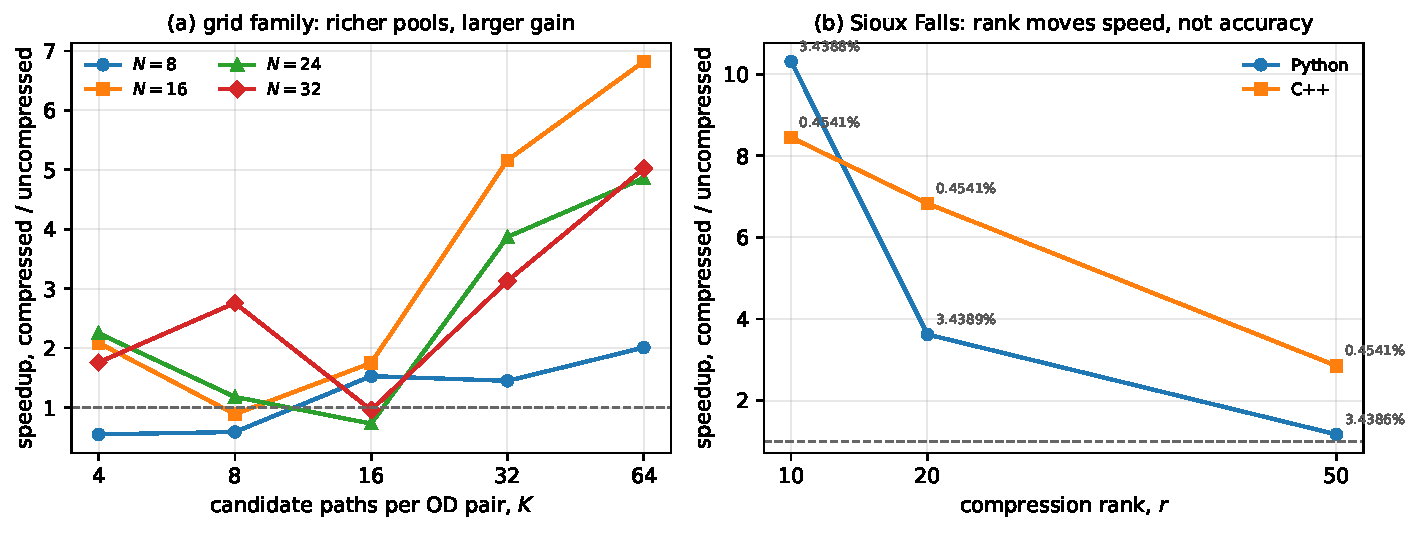
\includegraphics[width=\textwidth]{fig/fig_speedup_mechanisms.pdf}
\caption{The two mechanisms that govern the compression speedup. (a) On the grid
family, the gain grows with the depth of the candidate pool at every grid size, because the
uncompressed problem grows with the pool while the compressed dimension does not; the dashed
line marks parity. (b) On Sioux Falls the rank moves the speedup by close to an order of
magnitude in both implementations while the feasible objective gap, annotated at each point,
is unchanged to four decimal places --- over this range the rank is a speed parameter, not an
accuracy parameter.}
\label{fig:speedup-mechanisms}
\end{figure}

\subsection{The Rank is a Speed Parameter}
\label{sec:rank}


Equation~\eqref{eq:cost-rule} predicts that the rank controls cost linearly. The submitted
study swept $r\in\{50,100,150,200\}$ and found solution quality insensitive to $r$ while cost
grew --- correct, but sampled entirely on the expensive side. Table~\ref{tab:impact-rank}
sweeps downwards on Sioux Falls in both implementations.

\begin{table}[h]
\centering
\caption{Effect of the rank on Sioux Falls ($\tau=600$, $91\%$ variable
reduction, matched tolerance, medians of three runs). Speedup is against each
implementation's own uncompressed baseline ($1.34$s Python, $8.20$s C\texttt{++}). The
feasible objective gap is unchanged to four decimal places across the entire range.}
\label{tab:impact-rank}
{\small
\begin{tabular}{llrrr}
\toprule
Implementation & $r$ & CPU (s) & \textbf{Speedup} ($\times$) & Feasible obj.\ gap (\%)\\
\midrule
Python & 10 & 0.13 & \textbf{10.31} & 3.4388\\
       & 20 & 0.37 & \textbf{3.62}  & 3.4389\\
       & 50 & 1.15 & \textbf{1.17}  & 3.4386\\
\midrule
C\texttt{++} & 10 & 0.97 & \textbf{8.45} & 0.4541\\
             & 20 & 1.20 & \textbf{6.83} & 0.4541\\
             & 50 & 2.88 & \textbf{2.85} & 0.4541\\
\bottomrule
\end{tabular}}
\end{table}

The speedup varies by nearly an order of magnitude while the feasible objective gap moves in
the fourth decimal place (Figure~
ef{fig:speedup-mechanisms}b). Over this range the rank is therefore almost purely a speed
parameter: it multiplies the dense reconstruction without moving the solution. The optimum is
interior rather than at $r\to0$, because too small a subspace eventually lengthens the inner
solves --- visible on the grid, where $N=16$, $K=32$ gives $5.24\times$, $7.34\times$ and
$5.44\times$ at $r=10$, $20$ and $40$. Combining this with \eqref{eq:cost-rule} gives the
design rule used throughout the rest of the study: \emph{choose $2r$ no larger than the
average path length}, which on these instances means $r\approx10$--$20$ rather than the
$r=50$ of the submitted experiments. Section~\ref{sec:road-networks} quantifies what that
choice is worth on a road network.

\conoteY{This rule is the direct answer to Referee~2's request for analytical guidance on
$r$, and it is currently the only place we give a parameter rule. He asked the same question
about $\tau$ --- uniform or per-OD, and how it relates to convergence --- and we still choose
$\tau$ by quantile with no argument. If you can supply even a heuristic derivation for $\tau$
analogous to \eqref{eq:cost-rule}, it would close his second objection as cleanly as this
closes the first.}


\subsection{Which Subspace to Keep: Flow-Weighted Selection}
\label{sec:weighted-basis}

Section~\ref{sec:rank} fixes how large the retained subspace should be. A separate question is
which subspace of that size to retain. The natural answer, and the one used above, is the
leading left-singular subspace of $B_2$, which minimises $\|B_2 - \Pi B_2\|_F$. That criterion
counts every minor path equally, and it is not the criterion the problem asks for: a minor path
enters the link load in proportion to the flow it carries, so an error on a path carrying a
thousand vehicles matters a thousand times more than the same error on a path carrying one.

Replacing $B_2$ by $\operatorname{diag}(\sqrt{w_0})\,B_2$ before the factorisation retains
instead the subspace minimising $\sum_p w_{0,p}\|(B_2-\Pi B_2)_p\|^2$, so the rank budget is
spent where the flow is. The two factorisations are the same size and cost the same --- $0.94$s
against $0.97$s on Chicago Sketch at $r=20$ --- so any difference in solution time is a
convergence effect and not preprocessing overhead. Table~\ref{tab:weighted-basis} varies the
candidate pool at fixed network, demand, threshold and rank.

\begin{table}[h]
\centering
\caption{Effect of flow-weighted subspace selection on Chicago Sketch ($\tau=4.54$, $r=20$,
matched tolerance). Network, demand and parameters are fixed; only the richness of the
candidate pool varies. Both bases are solved back to back on each instance.}
\label{tab:weighted-basis}
{\small
\begin{tabular}{rrrrrr}
\toprule
& \multicolumn{2}{c}{flow-weighted} & \multicolumn{2}{c}{plain} & \\
\cmidrule(lr){2-3}\cmidrule(lr){4-5}
$\bar K$ & speedup & gap (\%) & speedup & gap (\%) & gap reduction\\
\midrule
2.45  & \textbf{1.62} & \textbf{0.0284} & 1.55 & 0.0291 & $-2.4\%$\\
3.49  & \textbf{3.71} & \textbf{0.0202} & 3.34 & 0.0232 & $-12.9\%$\\
8.64  & \textbf{1.55} & \textbf{0.2086} & 1.34 & 0.7024 & $\mathbf{-70.3\%}$\\
11.09 & \textbf{0.83} & \textbf{0.4350} & 0.66 & 1.1914 & $\mathbf{-63.5\%}$\\
15.34 & \textbf{1.20} & \textbf{0.8649} & 1.15 & 1.8651 & $\mathbf{-53.6\%}$\\
\bottomrule
\end{tabular}}
\end{table}

\textbf{The effect is on accuracy, and only on accuracy.} The gap column improves at every
richness point, by more than half wherever $\bar K \ge 8.64$, and these figures are exact:
feasible objective gaps are deterministic and reproduce bit for bit across runs. The speedup
column moves in the same direction, but by margins of $4$ to $26\%$, which is inside the
measurement noise reported in Section~\ref{sec:setup}. Pooling all $34$ controlled
weighted-versus-plain pairs measured in this study --- each a single instance with both bases
solved back to back --- the gap improves in $27$, whereas the speedup improves by more than the
noise floor in only $2$. We therefore claim an accuracy improvement and explicitly do not claim
a speed improvement.

The trend across the table is the explanation: a rich candidate pool is rich precisely in paths
that carry almost no flow, and the unweighted criterion spends its rank budget representing
them. This is why the regime that was least favourable in Section~\ref{sec:road-networks} ---
rich pools, where the compressed problem showed the largest gap --- is the regime the weighting
repairs most.

The grid family reproduces the effect on the axis that can be resolved. Across its twenty cells
the weighted basis lowers the feasible gap in $15$, taking the mean from $1.285\%$ to
$1.112\%$, with the largest improvements again at high pool depth (at $N=32$, $K=64$ the gap
falls from $0.406\%$ to $0.000\%$). Sioux Falls, at $91\%$ variable reduction, shows the same
sign and the largest relative movement, $11$ to $20\%$. The conclusion is that weighting makes
the subspace criterion consistent with the objective --- the retained directions are the ones
that carry flow --- and that this buys accuracy at no preprocessing cost, not speed.

\subsection{The Affine Offset is Load-Bearing}
\label{sec:offset-study}


The representation is affine, $x_{\text{minor}}=w_0+U_rz$, and the offset $w_0$ is the
nominal minor flow. Because $U_r$ is signed, the feasible set $\{w_0+U_rz\ge0\}$ contains the
starting point $z=0$ in its interior only by virtue of $w_0$; without the offset, $z=0$ lies
on the boundary of every reconstructed row simultaneously. To test whether this matters we
remove the offset exactly --- setting $w_0=0$ while moving its flow into the base link volume
and the effective demand, so the model is unchanged --- and re-solve.

The effect is large. Across the twenty grid cells of Table~\ref{tab:grid-matrix} the mean
speedup falls from $2.60\times$ to $1.07\times$ and the mean feasible gap grows from $0.75\%$
to $2.42\%$; the cells where compression is strongest collapse ($N=24$, $K=64$ from
$4.86\times$ to $0.45\times$; $N=16$, $K=64$ from $6.82\times$ to $1.86\times$). On Sioux
Falls the compressed solve slows from $1.7$s to $7.9$s, a fall from $6.2\times$ to
$1.34\times$, with the cost per inner iteration rising fourfold at nearly unchanged iteration
count: with the hinge active at the iterate, the augmented Lagrangian subproblem becomes
nonsmooth exactly where the solver works. In the Python implementation the offset-free
variant is not slower, and the accuracy penalty appears only on the larger instances, so the
speed half of this conclusion is specific to the compiled solver while the accuracy half is
not. The offset is therefore not an implementation convenience: \emph{a signed subspace of
nonnegative flows is usable only relative to an interior anchor}, and $w_0$ supplies it.

The two representational choices are independent. Removing the offset from the
\emph{flow-weighted} representation of Section~\ref{sec:weighted-basis} degrades it by the same
mechanism and by a similar amount: across the grid family the mean feasible gap rises from
$1.112\%$ to $1.394\%$, and individual cells collapse in the same way (at $N=32$, $K=64$,
$5.41\times$ at a gap of $0.000\%$ becomes $1.00\times$ at $1.681\%$). Choosing the subspace
better does not remove the need for an anchor inside it, and choosing the anchor well does not
substitute for aligning the subspace with the flow. The two act on different parts of the
representation and their benefits do not overlap.

\conote{This result cuts both ways and we should decide how to present it. It explains why the
representation works, but it also quantifies the dependence Referee~1 objected to: $w_0$ is
obtained by solving the full problem, and we have now proved the method needs it. The
strongest available answer is an experiment we have not run --- reuse a \emph{stale} $w_0$
from a perturbed instance and show the speedup survives. That single test would answer the
circularity objection, the preprocessing objection and the ``which application setting''
objection at once. Recommend we run it before resubmission.}


\subsection{Which Operator Benefits from Compression}
\label{sec:operator-study}


The compressed representation is independent of the solution method, so one may ask whether
the benefit is a property of the representation or of the augmented Lagrangian. We solve the
same compressed instances with three operators: the augmented Lagrangian; gradient projection
on the compressed set; and a reduced-gradient method that eliminates OD conservation by
anchor substitution. Table~\ref{tab:operator-compression} reports the result on grid cells in
the regime where compression is effective.

\begin{table}[h]
\centering
\caption{Speedup from compression, by solution operator, on grid cells
(Python, $w_0$ representation, matched tolerance). Each column is the operator's own
uncompressed time divided by its compressed time. Frank--Wolfe has no compressed counterpart
because the linear oracle over the compressed set is itself a linear program.}
\label{tab:operator-compression}
{\small
\begin{tabular}{lrrr}
\toprule
Grid cell & ALM & Gradient projection & Reduced gradient\\
\midrule
$N=16$, $K=16$ & \textbf{1.11} & 0.00 & 0.07\\
$N=16$, $K=32$ & \textbf{1.22} & 0.01 & 0.26\\
$N=16$, $K=64$ & \textbf{1.96} & 0.01 & 0.13\\
$N=32$, $K=16$ & \textbf{3.85} & 0.02 & 0.34\\
$N=32$, $K=32$ & \textbf{1.74} & 0.04 & 0.22\\
$N=32$, $K=64$ & \textbf{2.54} & 0.10 & 0.26\\
\bottomrule
\end{tabular}}
\end{table}

Only the augmented Lagrangian benefits. The reason is structural rather than incidental. An
iteration costs gradient work over the \emph{variables} plus feasibility work over the
\emph{constraints}; compression reduces the former and, because the reconstruction is dense,
increases the latter. The augmented Lagrangian carries feasibility in the objective through
multipliers and a penalty, so its iteration cost is gradient-dominated and the variable
reduction passes through to wall-clock time. Gradient projection instead derives its speed
from a projection that is separable across OD pairs and available in closed form; on the
compressed set $\{A_1y+Mz=d_{\mathrm{eff}},\,y\ge0,\,w_0+U_rz\ge0\}$ the latent variables
$z$ appear in every OD equality and in every reconstructed bound, so separability is lost and
the projection degrades into a coupled quadratic program. On the road networks this is not
merely slower but infeasible: the exact projection requires a dense factorization of order
the number of OD pairs, which at $\ell=17{,}464$ does not scale. The reduced-gradient method
removes the OD equalities by substitution, but the binding cost is the dense reconstruction,
which substitution does not touch; what elimination removes, the representation restores.

We therefore state the scope explicitly: \emph{variable reduction accelerates a method whose
per-iteration bottleneck lies in the variables, not in the constraints.} This is the
measured justification for pairing the compressed representation with an augmented Lagrangian
rather than a projection-type method, and it is the reason the framework of
Section~\ref{sec:compression_framework} is built that way.

\conote{Referee~2 wrote that ``the augmented Lagrangian method is quite standard'' and wanted
a tailored algorithm. This subsection is our answer: not a new algorithm, but a demonstration
that the pairing is forced. Whether that satisfies him is the main uncertainty in the
revision. He also asked for comparison against state-of-the-art path-based methods; we compare
four operators but no bush-based method (Algorithm~B, OBA, iTAPAS). Do we add one, or argue
the comparison is out of scope?}


\subsection{Road Networks}
\label{sec:road-networks}


Three questions remain for the road networks: do the operators agree on the same answer; does
the richness prediction of \S\ref{sec:cost-model} hold on a real network; and what does the
rank rule of \S\ref{sec:rank} buy in practice.


\subsubsection*{Consistency of the operators}


Before comparing efficiency we verify that the methods share a numerical target.
Table~\ref{tab:operator-consistency} solves one instance with all operators under matched
tolerances and a common feasibility conversion.


\begin{table}[h]
\centering

\caption{Numerical consistency on Sioux Falls under matched stopping tolerances. The
reference is the best feasible point over the uncompressed operators (full-path gradient
projection, feasible objective $4.231\times10^{6}$, certificate $9.1\times10^{-10}$). The
augmented Lagrangian's feasibility-based stopping rule leaves it $0.048\%$ above that
reference; the near-agreement of all operators is the consistency this table quantifies.}
\label{tab:operator-consistency}
\resizebox{\textwidth}{!}{%
\begin{tabular}{llrrrrr}
\toprule
Representation & Method & Raw obj. diff. (\%) & $\|A\tilde x-d\|_\infty$ & $\delta_F$ (\%) & Feasible obj. gap (\%) & Link-flow diff. (\%)\\
\midrule
Full ($\tau=0$) & ALM & 0.048 & $8.7\times10^{-11}$ & $1.3\times10^{-9}$ & 0.048 & 1.156\\
Full ($\tau=0$) & Frank--Wolfe & $1.2\times10^{-4}$ & $2.4\times10^{-10}$ & $2.7\times10^{-12}$ & $1.2\times10^{-4}$ & $5.1\times10^{-4}$\\
Full ($\tau=0$) & Gradient projection & $9.8\times10^{-8}$ & $5.5\times10^{-11}$ & $1.5\times10^{-11}$ & $9.8\times10^{-8}$ & 0.005\\
\midrule
Compressed ($\tau=600$, $r=20$) & ALM & 3.489 & $1.7\times10^{-10}$ & $1.5\times10^{-5}$ & 3.489 & 4.679\\
Compressed ($\tau=600$, $r=20$) & Gradient projection (signed) & 3.308 & $7.8\times10^{-11}$ & 0.102 & 3.461 & 4.655\\
\bottomrule
\end{tabular}}

\end{table}


The compressed rows agree with each other to within $0.03$ percentage points of feasible
objective gap, confirming that the gap is a property of the representation at this
$(\tau,r)$ and not of the operator, while the uncompressed rows bracket the reference to
within $0.05\%$. Frank--Wolfe is the most accurate uncompressed operator at loose tolerance
and is used as an honest baseline where relevant.


\begin{table}[h]
\centering
\caption{Network characteristics. Singleton paths correspond to the OD pairs with a unique feasible path and are excluded from the compressed problem.}
\label{tab:network-characteristics}
{\small
\begin{tabular}{lrrr}
\toprule
 & Chicago Sketch & Chicago Regional & Philadelphia \\
\midrule
Nodes / Links & 933 / 2{,}950 & 12{,}982 / 39{,}018 & 13{,}389 / 40{,}003 \\
Multi-path variables ($n$) & 42{,}774 & 879{,}625 & 1{,}846{,}068 \\
Multi-path OD pairs ($\ell$) & 17{,}464 & 353{,}582 & 601{,}644 \\
Average paths per multi-path OD ($\bar K=n/\ell$) & 2.45 & 2.49 & 3.07 \\
Multi-path flow share & 23.5\% & 59.2\% & 70.9\% \\
\bottomrule
\end{tabular}
}
\end{table}

\subsubsection*{Route richness and the rank rule}


Table~\ref{tab:cutoff-summary} varies route richness on Chicago Sketch at fixed network and
demand, by enriching the candidate pool from the submitted $\bar K=2.45$ to $\bar K=15.34$,
and reports the same axis at the rank chosen by \S\ref{sec:rank} and at the submitted rank.

\begin{table}[h]
\centering
\caption{Route-richness axis on Chicago Sketch: same network and demand,
candidate pools of increasing average richness $\bar K$, $\tau=4.54$, Python implementation.
The $r=20$ column applies the rule of \S\ref{sec:rank}; the $r=50$ column is the submitted
rank, shown for comparison at identical accuracy.}
\label{tab:cutoff-summary}
{\small
\begin{tabular}{rrrrrrr}
\toprule
$\bar K$ & $\bar K/q$ & Full dim.\ $n$ & Compressed dim.\ $s+r$ & \textbf{Speedup} ($r=20$) & Speedup ($r=50$) & Feasible obj.\ gap (\%)\\
\midrule
2.45  & 2.14  & 42{,}774      & 20{,}017  & \textbf{1.17} & 0.98 & 0.03\\
3.49  & 3.37  & 229{,}175     & 67{,}986  & \textbf{4.84} & 1.95 & 0.02\\
8.64  & 7.77  & 709{,}567     & 91{,}297  & \textbf{1.00} & 0.66 & 0.72\\
11.09 & 9.84  & 903{,}516     & 91{,}780  & \textbf{0.74} & 0.67 & 1.18\\
15.34 & 13.21 & 1{,}323{,}999 & 100{,}185 & \textbf{1.07} & 0.67 & 1.88\\
\bottomrule
\end{tabular}}
\end{table}

Two readings. First, the rank rule is worth a factor of about $2.5$ at the peak --- $4.84
\times$ against $1.95\times$ --- at accuracy identical to two decimal places, so a
substantial part of the attainable speedup in the submitted study was lost to the rank
choice alone. Second, and unlike the grid, the speedup on Chicago Sketch is \emph{not}
monotone in richness: it peaks near $\bar K\approx3.5$ and settles close to unity beyond
$\bar K\approx9$, while the feasible gap grows from $0.03\%$ to $1.88\%$. Equation
\eqref{eq:cost-rule} explains the difference between the two families. Chicago Sketch paths
average about $15$ links, so even at $r=20$ the dense term $2r=40$ exceeds the sparse term;
grid paths at $N=32$ average $35$--$45$ links, and the inequality runs the other way. The
compression is thus best suited to networks with long paths and many parallel routes, and the
enriched-pool regime of a short-path network is its adverse case.

Applying the rank rule to the submitted threshold grid improves accuracy as well as time: at
$r=20$ the conversion $\delta_F$ vanishes at every threshold, the feasible objective gaps are
$0.027\%$, $0.000\%$, $0.020\%$ and $0.028\%$ for $\tau=0$, $0.46$, $1.06$ and $4.54$, and
the link-flow $R^2$ rises to between $0.9997$ and $1.0000$, compared with $0.990$--$0.996$ at
$r=50$. The distribution of demand between major and minor paths at each threshold is
reported in Appendix~\ref{app:pathflow}.

\conote{Chicago Regional and Philadelphia are not yet re-evaluated at the corrected rank. The
submitted Regional pool ($879{,}625$ paths) is no longer on file; the closest available
instance has $2{,}024{,}525$ paths and $30$ links per path, which by \eqref{eq:cost-rule}
should favour $r\approx10$. A C\texttt{++} rank-by-offset experiment on it is running.
Referee~1 will reasonably note that our largest speedups come from Sioux Falls and a synthetic
grid, so carrying at least one large road network at the corrected rank matters more than any
other remaining item.}


\subsection{Reading the Two Representational Choices Together}
\label{sec:tradeoff}

The subspace criterion and the affine offset act on different parts of the same representation,
and both were measured by the same device: an instance solved twice, back to back, with one
choice changed and everything else held fixed. Figure~\ref{fig:paired} shows every such pair as
a displacement rather than as a point, which is the only form in which these comparisons are
controlled. The absolute position of a configuration in the speed--accuracy plane is dominated
by which instance it is; the displacement isolates the choice under study.

\begin{figure}[h]
\centering
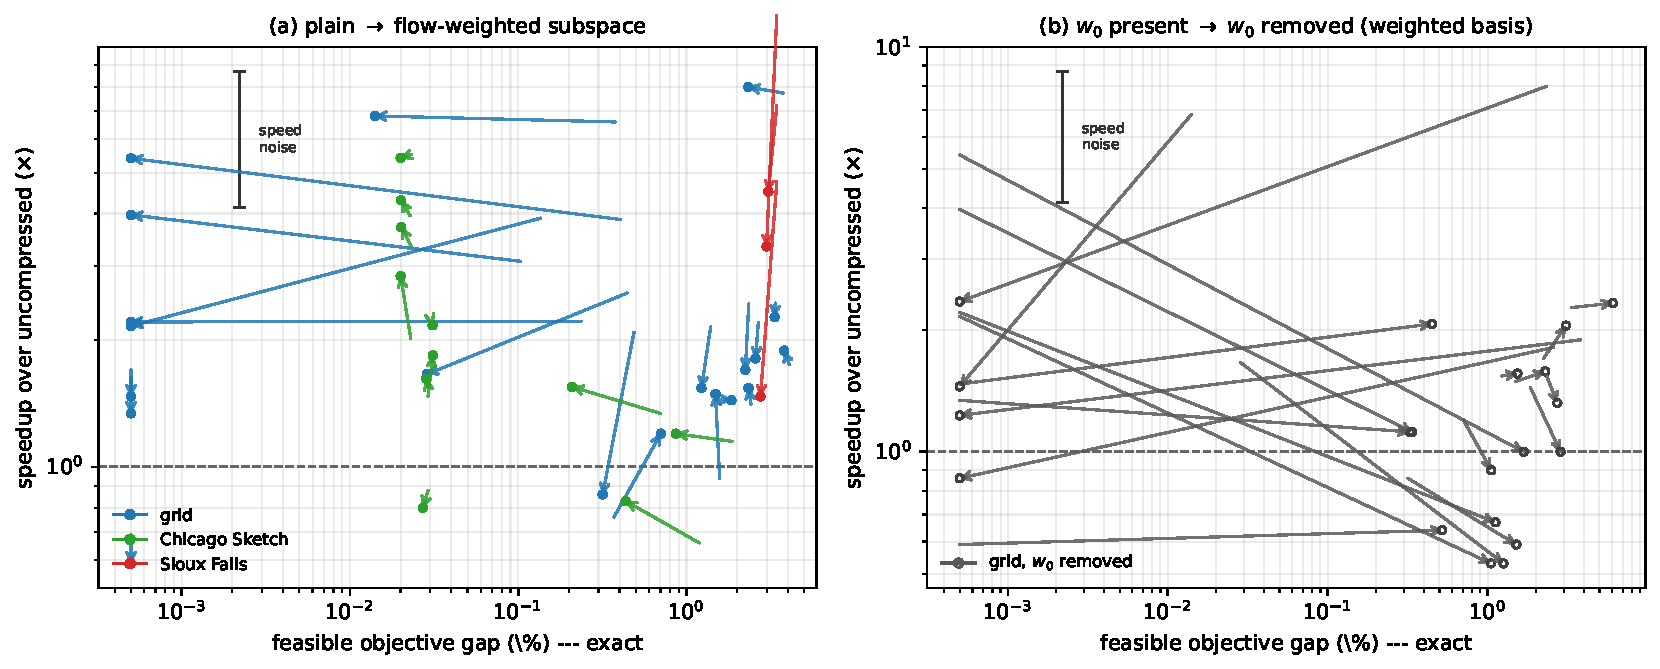
\includegraphics[width=\textwidth]{fig/fig_paired.pdf}
\caption{Paired comparisons. Each arrow is one instance solved twice with a single change,
running from the plain object to the one advocated here: (a) plain to flow-weighted subspace,
(b) no offset to offset present. Open markers are the baseline. The horizontal axis is exact;
the vertical axis carries the measurement noise of Section~\ref{sec:setup}, drawn as the error
bar, so vertical displacements shorter than it are not effects.}
\label{fig:paired}
\end{figure}

Comparing the two panels separates the two mechanisms cleanly, and the noise floor is what
makes the separation legible. In panel~(a) the arrows point left in $27$ of $34$ pairs, so the
weighted subspace improves accuracy, and that is measured exactly; vertically they scatter, and
only $2$ of $34$ rise by more than the noise floor, so we claim no speed effect for the
weighting. Panel~(b) behaves differently. Adding the offset improves the gap in $16$ of $20$
grid cells \emph{and} improves the solution time by more than the noise floor in $10$ of $20$.

The offset is therefore a speed mechanism as well as an accuracy one, whereas the subspace
criterion is an accuracy mechanism only. This is what one would expect from
Sections~\ref{sec:weighted-basis} and \ref{sec:offset-study}: weighting rotates the retained
subspace, changing what the representation can express but not how hard the subproblem is,
while the offset moves the starting point into the interior of the feasible set and so changes
the difficulty of the subproblem directly. The two act on different parts of the representation
and neither substitutes for the other.

Figure~\ref{fig:3d} shows the same two comparisons over the full grid design, on the axis that
can be resolved. The weighted sheet lies below the plain one and the offset-free sheet lies
above both, and the separation grows with pool depth, which is where the criterion has the most
to gain.

\begin{figure}[h]
\centering
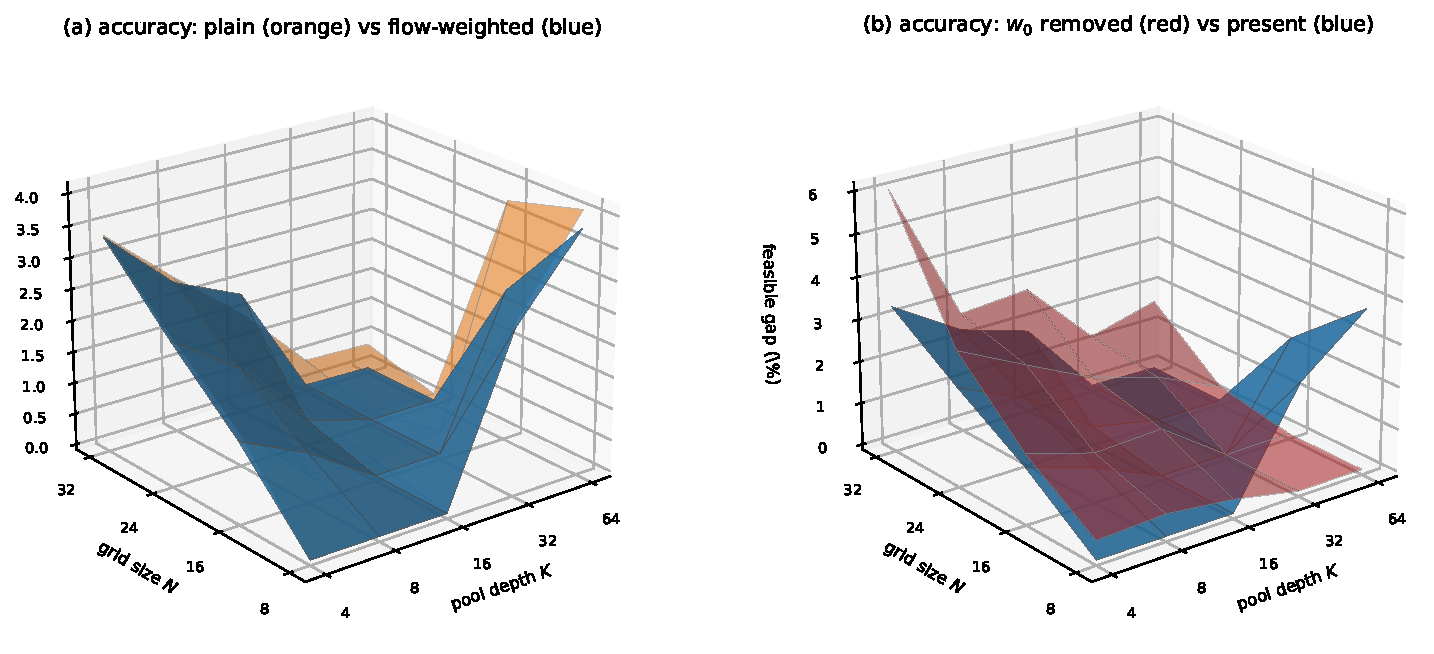
\includegraphics[width=\textwidth]{fig/fig_3d.pdf}
\caption{Feasible objective gap over the grid design $(N,K)$. (a) plain (orange) against
flow-weighted (blue): the weighted sheet is lower in $15$ of $20$ cells. (b) offset present
(blue) against removed (red): removing the anchor lifts the surface in $16$ of $20$ cells.}
\label{fig:3d}
\end{figure}



\subsection{Scope and Limitations}
\label{sec:scope-limits}


Four limitations bound the claims above, and each is a measurement rather than a caveat.

\emph{The speedup depends on the implementation.} On the richness axis of
Table~\ref{tab:cutoff-summary} the Python implementation peaks at moderate richness and falls
away, whereas the compiled implementation rises monotonically towards unity without crossing
it; the compiled solver's sparse kernels are relatively faster than its dense ones, which
moves the balance in \eqref{eq:cost-rule}. Sioux Falls is favourable in both ($3.6\times$ and
$6.2\times$). Speedup is therefore a property of representation, operator, implementation and
instance geometry jointly, and we report it only within an implementation.

\emph{The dense reconstruction is the binding constraint.} Reducing the number of independent
variables does not reduce the $n-s$ reconstructed inequalities. This is what
\eqref{eq:cost-rule} formalizes, what the falling branch of Table~\ref{tab:cutoff-summary}
measures, and what limits the method on short-path networks with rich pools.

\emph{A grouped representation removes that limit but is not yet faster.} Replacing the
signed subspace by nonnegative groups makes feasibility a bound constraint by construction,
with no reconstruction at all. Measured on the adverse cells of
Table~\ref{tab:cutoff-summary}, it is essentially exact --- feasible gaps of $0.016\%$ and
$0.000\%$, in one case improving on the uncompressed solution --- but in the present
implementation it is not faster. It is the natural representation for the regime where the
signed subspace struggles, and we leave its efficient implementation to future work.

\emph{Timing precision.} Large-instance timings are single runs; repeated identical solves
varied by up to $40\%$ under machine load, so ratios near unity on those instances should not
be read as ordered.


\section{Conclusion and Discussion}
\label{sec:conclusion}
{\color{red}
We developed an integrated compressed traffic assignment framework in which nominal path flows identify major paths, deviations of the minor-path flows are represented through the fixed map $w=w_0+\Phi_rz$, and the SVD choice $\Phi_r=U_r$ supplies the approximation used by the augmented Lagrangian implementation. The contribution is this unified compression-and-solution construction rather than the SVD or augmented Lagrangian principle in isolation.

The computational study is organized around a cost model rather than a parameter sweep. Because the reconstruction $w_0+U_rz\ge0$ is dense, a compressed gradient pays about $2r$ operations per minor path where the uncompressed gradient pays the length of a path, so compression reduces work when $2r$ is at most the average path length. A controlled grid family confirms the prediction, with speedups rising with candidate-pool depth to $6.8	imes$ at unchanged accuracy; a rank sweep shows that over the useful range the rank is almost purely a speed parameter, changing solution time by an order of magnitude while the feasible objective gap moves in the fourth decimal place; choosing the retained subspace by flow-weighted rather than plain reconstruction error reduces the feasible objective gap by more than half on route-rich instances at no additional preprocessing cost, an accuracy gain that the measurement precision resolves cleanly while the accompanying time differences do not; and an exact ablation shows that the affine offset is load-bearing, since a signed subspace of nonnegative flows is usable only relative to an interior anchor. These last two act on different parts of the representation and their benefits do not overlap. Comparing operators on the same compressed instances shows that the benefit is specific to the augmented Lagrangian: variable reduction accelerates a method whose per-iteration bottleneck lies in the variables, whereas projection- and reduced-gradient-type methods depend on a separable feasible set that compression destroys. This is the measured justification for the pairing developed in this paper.

The scope remains conservative. The reconstructed nonnegativity system contains path-scale components and $U_r$ is generally dense. The factored and mixed implementations show that this density did not eliminate per-inner-iteration savings in the tested regime, but total-time gains remain problem-dependent because compression can increase the iteration count. The framework is most appropriate when a path pool and nominal flow are available and related assignments allow the compression factors to be reused. Extensions requiring a different representation, adaptive path management, or other network-optimization domains are outside the scope of this paper.
}

\bibliographystyle{alpha}
\bibliography{ref} 


\appendix

\section{Notation}\label{app:notation}

\begin{longtable}{ll}
\caption{Summary of Main Notation} \label{tab:notation} \\
\toprule
Symbol & Description \\
\midrule
\endfirsthead
\toprule
Symbol & Description \\
\midrule
\endhead
\midrule
\endfoot
\bottomrule
\endlastfoot
\multicolumn{2}{l}{\textbf{Network and Demand}} \\
$d$ & OD demand vector (multi-path ODs only) \\
$v$ & Link flow vector \\
$v_0$ & Link flow from singleton paths \\
$m$ & Number of links \\
$n$ & Number of paths (excluding singletons) \\
$s$ & Number of major paths \\
$\ell$ & Number of multi-path OD pairs \\
\midrule
\multicolumn{2}{l}{\textbf{Path Variables}} \\
$x$ & Full path flow vector \\
$y$ & Major-path flow vector \\
$w$ & Minor-path flow vector \\
$w_0$ & Nominal minor-path flow vector \\
$z$ & Low-dimensional minor-path coordinate vector \\
\midrule
\multicolumn{2}{l}{\textbf{Incidence Matrices}} \\
$B$ & Path-link incidence matrix ($n \times m$)\\
$B_1$ & Incidence matrix for major paths ($s \times m$)\\
$B_2$ & Incidence matrix for minor paths [$(n-s) \times m$]\\
$A$ & OD-path incidence matrix ($\ell \times n$)\\
$A_1$ & OD-major-path incidence matrix ($\ell \times s$)\\
$A_2$ & OD-minor-path incidence matrix [$\ell \times (n-s)$]\\
$D = B_2'U_r$ & Compressed link matrix ($m \times r$) \\
$M = A_2 U_r$ & Compressed OD matrix ($\ell \times r$) \\
\midrule
\multicolumn{2}{l}{\textbf{Low-Rank Compression}} \\
$B_2 \approx U_r \Sigma_r V_r'$ & Rank-$r$ truncated SVD of minor-path matrix \\
$U_r$ & Rank-$r$ left singular basis for minor paths \\
$r$ & Compression rank \\
$w_0+U_r z$ & Affine compressed minor-path flow representation \\
$\bar d=d-A_2w_0$ & OD demand remaining after the nominal minor-path contribution \\
\midrule
\multicolumn{2}{l}{\textbf{Optimization and ALM}} \\
$\hat{f}(y,z) = f(B_1'y + Dz + B_2'w_0 + v_0)$ & Compressed objective function \\
$\lambda$ & Lagrange multiplier vector (OD equality constraints) \\
$\mu$ & Lagrange multiplier vector (nonnegativity of $w_0+U_rz$) \\
$c = (c_1, c_2)$ & Component-wise penalty parameters \\
$\beta$ & Penalty growth factor \\
$\gamma$ & Penalty update threshold \\
\end{longtable}

\section{Path and Flow Distribution Tables}
\label{app:pathflow}
 
This appendix reports how demand splits between major and minor paths at each cutoff threshold. The three networks display markedly different concentration profiles. 

On Chicago Sketch (Table~\ref{tab:pathflow-sketch}), major paths carry roughly 23\% of total demand across all thresholds and minor-path flow stays below 1.5\% even at the most aggressive cutoff, indicating that the vast majority of demand is absorbed by singleton OD pairs that lie outside the compressed problem. On Chicago Regional (Table~\ref{tab:pathflow-regional}), major paths carry 47--59\% of demand, with minor-path flow rising to 11.7\% at $\tau = 1.033$; the heavier tail makes this network the most sensitive to the choice of $\tau$. On Philadelphia (Table~\ref{tab:pathflow-philly}), major paths dominate at 63--71\% of demand and minor-path flow reaches 7.8\% at $\tau = 5.3344$. In all three networks, the fraction of flow routed through minor paths grows smoothly with $\tau$, confirming that the cutoff acts as a continuous control over the major/minor partition rather than a sharp threshold.
 
\begin{table}[ht]
\centering
\caption{Path and Flow Distribution (Chicago Sketch)}
\label{tab:pathflow-sketch}
{\small\begin{tabular}{rrrrr}
\toprule
$\tau$ & $s$ & $n - s$ & Major Flow (\%) & Minor Flow (\%) \\
(veh) & (major) & (minor) & & \\
\midrule
0.000 & 42{,}774 & 0 & 267{,}805.15 (23.5) & 0.00 (0.0) \\
0.139 & 40{,}243 & 2{,}531 & 267{,}509.30 (23.5) & 295.85 (0.0) \\
0.341 & 32{,}650 & 10{,}124 & 265{,}813.58 (23.4) & 1{,}991.57 (0.2) \\
1.055 & 25{,}057 & 17{,}717 & 261{,}257.02 (23.0) & 6{,}548.13 (0.6) \\
4.541 & 19{,}995 & 22{,}779 & 250{,}289.70 (22.0) & 17{,}515.45 (1.5) \\
\bottomrule
\end{tabular}}
\end{table}
 
\begin{table}[ht]
\centering
\caption{Path and Flow Distribution (Chicago Regional)}
\label{tab:pathflow-regional}
{\small\begin{tabular}{rrrrr}
\toprule
$\tau$ & $s$ & $n - s$ & Major Flow (\%) & Minor Flow (\%) \\
(veh) & (major) & (minor) &  &  \\
\midrule
0.000 & 879{,}625 & 0 & 778{,}822.96 (59.2) & 0.00 (0.0) \\
0.126 & 827{,}019 & 52{,}606 & 772{,}855.35 (58.7) & 5{,}967.60 (0.5) \\
0.227 & 669{,}208 & 210{,}417 & 745{,}814.50 (56.7) & 33{,}008.46 (2.5) \\
0.460 & 511{,}394 & 368{,}231 & 694{,}810.96 (52.8) & 84{,}011.99 (6.4) \\
1.033 & 406{,}187 & 473{,}438 & 624{,}290.35 (47.4) & 154{,}532.61 (11.7) \\
\bottomrule
\end{tabular}}
\end{table}
 
\begin{table}[ht]
\centering
\caption{Path and Flow Distribution (Philadelphia)}
\label{tab:pathflow-philly}
{\small\begin{tabular}{rrrrr}
\toprule
$\tau$ & $s$ & $n - s$ & Major Flow (\%) & Minor Flow (\%) \\
(veh) & (major) & (minor) &  &  \\
\midrule
0.0000 & 1{,}846{,}068 & 0 & 10{,}157{,}630.99 (70.9) & 0.00 (0.0) \\
0.1610 & 1{,}721{,}624 & 124{,}444 & 10{,}141{,}117.22 (70.8) & 16{,}513.78 (0.1) \\
0.4473 & 1{,}348{,}298 & 497{,}770 & 10{,}037{,}598.50 (70.1) & 120{,}032.49 (0.8) \\
0.9866 & 1{,}099{,}414 & 746{,}654 & 9{,}867{,}685.32 (68.9) & 289{,}945.67 (2.0) \\
2.4435 & 850{,}528 & 995{,}540 & 9{,}481{,}879.91 (66.2) & 675{,}751.08 (4.7) \\
5.3344 & 726{,}087 & 1{,}119{,}981 & 9{,}036{,}971.50 (63.1) & 1{,}120{,}659.49 (7.8) \\
\bottomrule
\end{tabular}}
\end{table}
 
 
\end{document}
